%%%%%%%%%%%%%%%%%%%%%%%%%%%%%%%%%%%%%%%%%%%%%%%%%%%%%%%%%%%%%%%%%%%%%%%%%%%%%%%%
%%                                                                
%%      SWSC LaTeX class for Journal of Space Weather and Space Climate
%%      
%%                                      (c) Springer-Verlag HD
%%                                      revised by EDP Sciences
%%                                      further revised by J. Watermann 
%%
%%%%%%%%%%%%%%%%%%%%%%%%%%%%%%%%%%%%%%%%%%%%%%%%%%%%%%%%%%%%%%%%%%%%%%%%%%%%%%%%
%%
%%      This demonstration file was derived from aa.dem
%%  
%%      AA vers. 7.0, LaTeX class for Astronomy & Astrophysics
%%      demonstration file
%%                                                (c) Springer-Verlag HD
%%                                                revised by EDP Sciences
%%
%%%%%%%%%%%%%%%%%%%%%%%%%%%%%%%%%%%%%%%%%%%%%%%%%%%%%%%%%%%%%%%%%%%%%%%%%%%%%%%%
%%
%%      modified for Journal of Space Weather and Space Climate
%%      by Jurgen Watermann, Editorial Advisor to SWSC
%%
%%      01-04-2012 original version
%%      02-04-2012 revision 1
%%      12-07-2012 revision 2
%%      06-12-2012 revision 3 
%%      01-01-2014 revision 4
%%      05-03-2016 revision 5
%%      11-05-2018 revision 6  (equations and figure captions line numbered)
%%
%%%%%%%%%%%%%%%%%%%%%%%%%%%%%%%%%%%%%%%%%%%%%%%%%%%%%%%%%%%%%%%%%%%%%%%%%%%%%%%%
%%
%%      The two sub-figures referenced in this template are of eps and png type,
%%      respectively, in order to demonstrate the usepackages subfigure and
%%      epstopdf and thus create pdf-only output 
%%
%%      If you want to use TexLive or MikTex together with a bibtex bibliography 
%%      file you may run Latex2e from the command line 
%%          pdflatex -shell-escape swsc.tex
%%          bibtex swsc (do not include an extension such as .tex or .bib)
%%          pdflatex -shell-escape swsc.tex
%%          pdflatex -shell-escape swsc.tex
%%
%%      A double call to pdflatex after calling bibtex is necessary in order to
%%      set citations and references correctly and insure that foreward/backward  
%%      linkage (backref option) is properly applied
%%      If you use MikTex you may need to make a triple call to pdflatex
%%
%%      If you are using TexLive or MikTex but not a bibtex type of bibliography
%%      you may simply run Latex2e twice from the command line 
%%          pdflatex -shell-escape swsc.tex
%%          pdflatex -shell-escape swsc.tex
%%
%%%%%%%%%%%%%%%%%%%%%%%%%%%%%%%%%%%%%%%%%%%%%%%%%%%%%%%%%%%%%%%%%%%%%%%%%%%%%%%%
%%
%%   single column 12-point version for review
%%

%%  with traditional abstract
\documentclass[referee,a4paper,12pt,traditabstract]{swsc} 

%%  with structured abstract 
%\documentclass[referee,a4paper,12pt,structabstract]{swsc} 
\usepackage{graphicx}
\usepackage{txfonts}
\usepackage{subfigure}
\usepackage{epstopdf}
\usepackage[displaymath,mathlines]{lineno}
\usepackage[authoryear,round]{natbib}
\usepackage[backref]{hyperref}
\usepackage{url}
\usepackage{pdfpages}
\usepackage[inline]{trackchanges}
%%    This version assumes using bibtex with the swsc bibliography style file
%\bibliographystyle{swsc}
\usepackage[none]{hyphenat}
\hypersetup{colorlinks=true,citecolor=cyan,urlcolor=cyan,linkcolor=blue}
\usepackage[]{xcolor}
%%    This version assumes using bibtex with the swsc bibliography style file
\bibliographystyle{swsc}

\hypersetup{colorlinks=true,citecolor=cyan,urlcolor=cyan,linkcolor=blue}

%%%%%%%%%%%%%%%%%%%%%%%%%%%%%%%%%%%%%%%%%%%%%%%%%%%%%%%%%%%%%%%%%%%%%%%%%%%%%%%%%%%%%%%%%%%%%%%%
\definecolor{CASIIlightindago}{RGB}{60,100,120}
\definecolor{CASIIdarkyellow}{RGB}{188,161,54}
\definecolor{CASIIdarkgreen}{RGB}{75,85,50}
\definecolor{CASIIaliceblue}{RGB}{16,120,150}

\begin{document}

\begin{linenumbers}  

   \title{Tracking usability and progress across disciplines: The evolution of TRLs to AULs.}

   \titlerunning{TRLs $\rightarrow$ AULs}

   \authorrunning{Alexa J. Halford}

   \author{A. J. Halford \inst{1} \and A. G. Burrell \inst{2} \and S. Elvidge \inst{3} \and J. Klenzing \inst{1} \and S. Bingham \inst{4}
          }

   \institute{1: NASA Goddard, Greenbelt MD, USA:
              \email{Alexa.J.Halford@nasa.gov} \\
2: US Naval Research Laboratory, Washington DC, USA: 
              \email{angeline.burrell@nrl.navy.mil} \\
3: SERENE, University of Birmingham, UK :
            \email{s.elvidge@bham.ac.uk}\\
4: Met Office, Fitzroy Road, Exeter, Devon, EX1 3PB, UK. 
}



  \abstract
 %% context heading (optional). leave {} empty if necessary  
   {We need to show these examples to convince ESA to use AULs}        %% replace by pair of curly brackets, {}, if structured abstract is selected
   

   \keywords{Tracking usability --
                Validation --
                Verification
               }

   \maketitle
%%
%%________________________________________________________________
%Perhaps another title taken from an article in the innovation journal ("From NASA to EU: the evolution of the TRL scale in Public Sector Innovation"  The Innovation Journal: The Public Sector Innovation Journal, Volume 22(2), 2017, article 3.) - From NASA to the EU - The evolution of the TRL framework to the AULs. 


As you add/agree/discuss the paper please feel free to add you name to the author list and your institution as well. Also feel free to add/edit/change the paper as you feel. 

\section{The need for a generalized tracking system to work across project type}
Tracking a project or team's productivity, progress, and usefulness can help with management of institutions and programs. Having metrics which are easy to use and interpret can help determine the success of a program, identify where roadblocks exist, and help plan for future directions and resources which may be needed. Using a single framework can ensure clear communication when reporting progress across programs and project types. When comparing two or more projects for a specific use (i.e. same application and requirements), using a single framework ensures consistency with understanding of each projects current progress. It has the added benefit of not having to learn new frameworks when moving to a new project. However, it is imperative that the framework used works for all groups and projects within the institution. If not all groups are able to achieve a "top grade",  bias can occur with the implication that not all groups are being productive. 

\subsection{Definitions and terminology}

We need to identify what, if any, terms are perhaps needed to be defined and/or are used differently by the Engineers, Software guys, and the research community. 

\subsection{The TRL framework }

\begin{table}
\caption{A brief description of the TRL phases and levels}
\centering
\begin{tabular}{ll}\hline
 TRL & Level description \\
 \hline
 \textcolor{black}{1}& \textcolor{black}{Basic principles observed and reported}\\
 \textcolor{black}{2} & \textcolor{black}{Technology concept or application formulated}\\ 
\textcolor{black}{3} &\textcolor{black}{Concept or application proven through analysis and experimentation} \\

\textcolor{black}{4}& \textcolor{black}{Basic prototype validated in laboratory environment}\\
 \textcolor{black}{5} & \textcolor{black}{Basic prototype validated in relevant environment}\\ 
 \textcolor{black}{6} &\textcolor{black}{System or subsystem model or prototype demonstrated in a relevant environment} \\

 \textcolor{black}{{7}}& \textcolor{black}{{System prototype demonstrated in a relevant environment}}\\
 \textcolor{black}{{8}} & \textcolor{black}{{Actual system completed and qualified for flight through test and demonstration}}\\ 
 \textcolor{black}{{9}} &\textcolor{black}{{Actual system proven through successful operation}} \\
\label{Tab_TRL}
\end{tabular}
\end{table}

One of the first frameworks developed to communicate the progress/readiness of a project for a specific application was the Technology Readiness Levels (TRL)  \citep{mankins1995technology} (European Space Agency (ESA) TRL definitions can be found at http://sci.esa.int/sci-ft/50124-technology-readiness-level/ and are summarized in Table \ref{Tab_TRL}). This framework allows for tracking the readiness of flight hardware for use in space. With the success of this framework, institutions have attempted to apply TRLs to many other types of projects, including non-hardware, non-space flight projects. Below, and in Table \ref{Tab_TRL} we summarize the TRLs and their requirements:  

\begin{description}
{\bf \item[TRL 1 -] Basic principles observed and reported.} Basic scientific research that can be turned into an application or a concept under a research and development program is considered.

{\bf \item[TRL 2 -] Technology concept or application formulated.} An idea is proposed for the practical application of current research, but there are no experimental proofs or studies to support the idea.

{\bf \item[TRL 3 -]  Concept or application proven through analysis and experimentation.} Active research and development begins, including analytical laboratory-based studies to validate the initial idea, providing an initial "proof of concept."

{\bf \item[TRL 4 -] Basic prototype validated in laboratory environment.} Basic examples of the proposed technology are built and put together for testing to offer an initial vote of confidence for continued development.

{\bf \item[TRL 5 -] Basic prototype validated in relevant environment.} More realistic versions of the proposed technology are tested in real-world or near real-world conditions, which includes initial integration at some level with other operational systems.

{\bf \item[TRL 6 -] System or subsystem model or prototype demonstrated in a relevant environment.} A near final version of the technology in which additional design changes are likely is tested in real-life conditions.

{\bf \item[TRL 7 -] System prototype demonstrated in a relevant environment.} The final prototype of the technology that is as close to the operational version as possible at this stage is tested in real-life conditions.

{\bf \item[TRL 8 -] Actual system completed and qualified for flight through test and demonstration.} The technology is thoroughly tested and no further major development of the technology is required. Its operation as intended is demonstrated without significant design problems.

{\bf \item[TRL 9 -] Actual system proven through successful operation.} The technology is deployed, and used, in an operational setting.
\end{description}

\subsection{Why TRLs don't work for all types of projects}

The TRL framework was designed specifically for spacecraft and instruments/software which would fly in space. This can be seen in how the requirements are written to reach a specific level as defined in \citet{mankins1995technology} and provided at ESA https://ecss.nl/home/ecss-e-hb-11a-technology-readiness-level-trl-guidelines-1-march-2017/. As an example, TRL 8's requirements are written as "Actual system completed and qualified for flight through test and demonstration". The initial TRL framework was designed to be high level and general to allow for flexibility between space instrumentation projects but still targeted specifically for space hardware components. While it is important to keep a framework such as TRLs general enough to be applied to many different types of projects, it is also useful to acknowledge what types of metrics and requirements need to be completed to achieve each stage resulting in a product which will have an added benefit to the user. However, by having requirements \change[Jeff]{such as TRL 8}{written using space-flight metrics as above}, projects which are not expected to go into space cannot reach the higher levels and thus cannot be identified as TRL 9. 

At the same time, the generality of other TRLs do not guarantee that the project will fulfill the needs of the end user.
This is especially true as the TRLs do not specify identifying metrics, requirements, or communication with an identified user.
This leads to several challenges of TRL implementation as reported by \citet{Olechowski2015} -- notably  subjectivity of the assessment and imprecision of the scale across projects.  
This limits the types of projects which can use the TRL scale to communicate their progress to becoming operational and useful to the identified user or user community. 

\subsection{Brief intro into the AULs}
   
\begin{figure}
\centering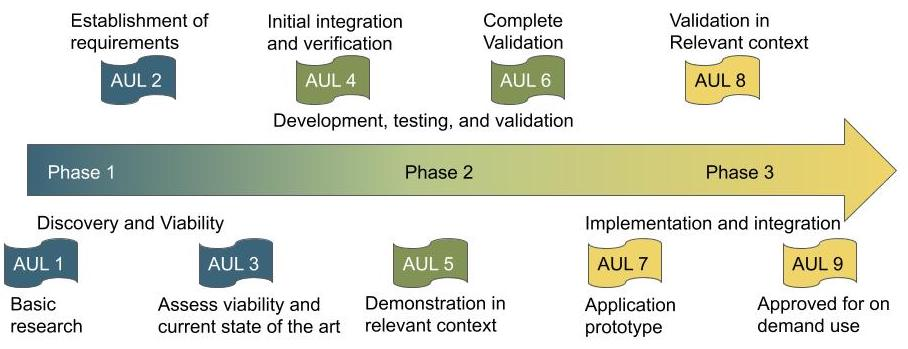
\includegraphics[width=0.9\linewidth]{Fig_AUL.jpg}
\caption{From \citet{halford19}: Application Usability Level (AUL) diagram showing how a project progresses towards an application from AUL 1 to AUL 9. A project will then pass through three main phases: discovery, development, and implementation as described in \citet{halford19}.}\label{Fig_AUL}
\end{figure}

The space weather community identified a need for a framework to help communicate the needs of a user to the researcher. This framework would then ensure that a project was correctly targeted and produce a usable product. While the TRL framework was considered, it was found to not adequately communicate the usability of a project for research, forecasting applications, or space weather tool development. The effort to create such a framework which would benefit these wide varieties of projects resulted in the Application Usability Levels (AULs) described in \citet{halford19} and \citet{cid2020} and  summarized in Figure \ref{Fig_AUL} and Table \ref{Tab_AUL}. The AUL framework focuses on clear communication between the team developing the tool or project for a specific application and their identified user. Focusing on communication ensures that the project will meet the needs and requirements of the user. Benefits to using the AUL framework include improving access to collaborators, project transparency, and communication of project results. Although milestones are identified in each of the levels, they are written in a general format to allow flexibility between individual projects, and types of projects, e.g. hardware, software, or research projects. 
   
Like the TRLs, the AULs have 9 levels. These 9 levels are then divided into three phases. Phase 1 is focused on Discovery and Viability. Within the first three levels basic research and development is completed. The end user is identified and the requirements for the project are established. Finally, the viability and feasibility of the project is assessed prior to moving ahead to Phase 2. Phase 2 is where development, testing, and validation are completed. This includes integration, validation, and demonstration of the project working within the relevant context. Phase 3 concludes the project with it's implementation and integration into the operational context.  

\begin{table}
\caption{A brief description of the AUL phases and levels}
\centering
\begin{tabular}{llll}\hline
Phase & Phase definition & AUL & Level description \\
 \hline
 & & \textcolor{CASIIaliceblue}{1}& \textcolor{CASIIaliceblue}{Basic research}\\
 \textcolor{CASIIaliceblue}{{\bf Phase 1} }& \textcolor{CASIIaliceblue}{{\bf Discovery and Viability }} & \textcolor{CASIIaliceblue}{2} & \textcolor{CASIIaliceblue}{Establishment of users and their requirements}\\ 
& & \textcolor{CASIIaliceblue}{3} &\textcolor{CASIIaliceblue}{Assess viability and current state of the art} \\
 \hline
 \hline
 & & \textcolor{CASIIdarkgreen}{4}& \textcolor{CASIIdarkgreen}{Initial integration and verification}\\
 \textcolor{CASIIdarkgreen}{{\bf Phase 2} }& \textcolor{CASIIdarkgreen}{{\bf Development, Testing,  }} & \textcolor{CASIIdarkgreen}{5} & \textcolor{CASIIdarkgreen}{Demonstration in the relevant context}\\ 
& \textcolor{CASIIdarkgreen}{{\bf and Validation}}& \textcolor{CASIIdarkgreen}{6} &\textcolor{CASIIdarkgreen}{Completed validation} \\
 \hline 
 \hline
 & & \textcolor{CASIIdarkyellow}{{7}}& \textcolor{CASIIdarkyellow}{{Application prototype}}\\
 \textcolor{CASIIdarkyellow}{{{\bf Phase 3}}}& \textcolor{CASIIdarkyellow}{{{\bf Implementation and Integration}}} & \textcolor{CASIIdarkyellow}{{8}} & \textcolor{CASIIdarkyellow}{{Validation in relevant context}}\\ 
& \textcolor{CASIIdarkyellow}{{{\bf into Operation}}} & \textcolor{CASIIdarkyellow}{{9}} &\textcolor{CASIIdarkyellow}{{Approved for on-demand use}} \\


\label{Tab_AUL}
\end{tabular}
\end{table}


\subsection{Mapping the TRLs to the AULs}
The AULs were developed and modified from the Application Readiness Levels (ARL) used by the Applied Science Program in NASA's Earth Sciences Division \cite[see Figure 1, or https://www.nasa.gov/sites/default/files/files/ExpandedARLDefinitions4813.pdf]{Pulkkinen2017}, and the TRL frameworks. Lesson's learned were adapted, along with input from across the space weather community to make sure this new framework would work for a wide variety of projects. This also ensures that projects which used the ARL and TRL framework would be able to use the AUL framework. 

Perhaps the primary difference between AULs and TRLs is the identification of a user. The user for a flight hardware project may be the funding institution, the researchers, and/or the satellite bus itself. The user, or set of users would be the group of people who would be identifying the requirements for the hardware. This may include the project manager (high level requirements), systems engineers (interface, payload restrictions), and members of the science team (range, accuracy, precision, and cadence of measured parameters).
Since each step of the AUL process requires communication between the end users and technology developers, the level identification process \annote[Jeff]{is transformed from a monologue to a dialogue}{Too harsh? Or accurate?}\annote[Alexa]{ and at times a broader conversation.}{I think that this is a very true statement. I don't think it reads too harsh but others should chime in.}\annote[Sean]{Not too harsh in my opinion.}

\subsubsection{TRL 1: Basic principles observed and reported/ AUL 1: Basic Research}
For both TRLs and AULs this initial level identifies that there is a possibility that the research can be turned into a useful application. The AUL milestones within here are: \\

\noindent {\bf Milestones:}
\renewcommand{\labelenumi}{\alph{enumi})}
\begin{enumerate}
\item  Basic research is documented and disseminated for the project, so that the usability may be assessed by way of the AUL method. 
\item  Ideas for how the project output(s) may enhance decision making or be applied to an end user application are generated.
\item  Potential interested users are identified, but not necessarily contacted.  This could occur, for example, through a literature search, conference attendance, or workshop participation.
\end{enumerate}

\subsubsection{TRL 2: Technology concept or application formulated/ AUL 2: Establishment of users and their requirements for a specific application}
Within this level for both the AULs and TRLs there is a formalization of the project's concept. The AULs go a bit further with identifying and establishing communication between the researcher and the user as well as identifying the requirements and metrics necessary for a successful application as can be seen in the following AUL milestones: \\

\noindent {\bf Milestones:}
\begin{enumerate}
\item Decide on the user(s), contact the user(s), and establish a reliable channel of communication that is used at a suitable frequency.
\item Formalization of the application and project concept.
\item Identification and formalization of the requirements and metrics necessary for successful application of the project for the user's needs. 
\end{enumerate}

\subsubsection{TRL 3: Concept or application proven through analysis and experimentation/ AUL 3: Assess viability of concept and current state of the art }
Both TRL 3 and AUL 3 are focused on showing the feasibility and viability of the project. Within the AUL framework the milestones ensure the documentation of the proposed advancement, show a baseline performance, as well as identify current limitations as stated below: \\

\noindent {\bf Milestones:}
\begin{enumerate}
\item Documentation and dissemination of the project's expected advancements from the current state-of-the-art used towards the identified application along with the proposed metrics for the specified application. 
\item Perform the initial analysis of the individual project components, to determine the viability and feasibility of the entire project.
\item Complete a detailed characterization of the baseline performance and limitations with respect to the application.
\item Determine the viability and feasibility of the proposed project towards improving upon the state of the art for the identified application. If the project is deemed not viable or feasible, the project is put on hold until the identified roadblocks are removed.
\end{enumerate}

%\subsection{\textcolor{CASIIdarkgreen}{Phase II: Development testing and validation}}
%In Phase I, the current state of the art is identified,  basic research into current limitations and expected areas for improvements are completed, initial communication with the end user is established, and a proof-of-concept and show of viability  is made. Phase II  focuses on finalizing development of the new state-of-the-art project integrating the resulting tools into the identified applications, demonstrating the feasibility of the new product and validating the new system. 

\subsubsection{TRL 4: Basic prototype validated in laboratory environment/ AUL 4: Initial integration and verification}
Within both TRL 4 and AUL 4 the prototype is completed. The AULs have an additional milestone (shown below) where any organizational or human process issues/roadblocks are identified and managed. This ensures the feasibility of the project as it moves closer to completion. \\

\noindent {\bf Milestones:}
\begin{enumerate}
\item Integration of the individual components into the application.
\item Organizational challenges and human process issues (if applicable) are identified and managed. 
\end{enumerate}

\subsubsection{TRL 5: Basic prototype validated in relevant environment/ AUL 5: Demonstration in the relevant context}
The TRL 5 and AUL 5 requirements are to demonstrate and validate the prototype in the relevant environment/context. Below are the specific milestones for the AUL 5 requirements:\\

\noindent {\bf Milestones:}
\begin{enumerate}
\item The project team must articulate and disseminate the viability  for the improvement upon the state of the art.
\item Application components integrated into a functioning application system for use during the given relevant context parameters. 
\end{enumerate}

\subsubsection{TRL 6: System or subsystem model or prototype demonstrated in relevant environement/ AUL 6: Complete validation}
While in both TRL and AUL 5 the potential is articulated, in level 6 for both the TRL and AULS, the potential is fully demonstrated in the real-world or simulated operational environment and/or decision making context. The AULs have the additional milestone of requiring that the specific application and the metrics are documented as stated below. This ensures clear communication of the application and that the project meets the agreed upon metrics:\\

\noindent {\bf Milestones:}
\begin{enumerate}
\item Prototype application system beta-tested in a simulated operational environment.
\item Projected improvements in performance of the state-of-the-art and/or decision making activity demonstrated in simulated operational environment.  
\item Documentation and dissemination of the specific application and associated metrics and the projects progress towards this application.
\end{enumerate}

%\subsection{\textcolor{CASIIdarkyellow}{Phase III: Implementation and Integration into operational status}}
%While Phase I and II focused on the development and initial validation of the new model/data analysis effort for a specific application, Phase III is where it becomes handed off and fully integrated into the end user's application. This also includes new validation efforts to determine how well the new model/data analysis effort performs in a ``real world" setting. Validation and continued use in an operational environment drive the discovery of new scientific questions, problems, and new applications. Although this is the final phase for the current application with its specific requirements and metrics, the search for the next new and improved application continues. 

\subsubsection{TRL 7: System prototype demonstrated in a relevant environment/ AUL 7: Application prototype}
In TRL 7 and AUL 7, the product is fully moved and tested in the real-world or user environment.  A project is considered to have AUL 7 if the following milestones are achieved: \\

\noindent {\bf Milestones:}
\begin{enumerate}
\item The system must be fully integrated into the operational environment specified by the user. 
\item The system's functionality is tested and demonstrated in the user's specified relevant context. 
\item Project team must demonstrate the functionality of the new system for the user's application and disseminate the results.
\end{enumerate}

\subsubsection{TRL 8: Actual system completed and qualified for flight through test and demonstration/ AUL 8: Validation in relevant ``real world'' environment}

At TRL and AUL 8, the new project is fully integrated into the user application system and is initially validated by the user. The project is proven to work in its final form in the relevant context and operational environment, and no major changes should occur as it either meets or surpasses the identified requirements and metrics. While TRL8 specifies that the environment is space, the AULs are more general where the user defines the operational environment - which may be space, or their computer system. The AUL 8 milestones also require user documentation including verification and validation/metric results, any limitations of the new project, training documentation, and maintenance documentation as shown below. By including ideas for future developments, new projects and applications can be identified and lessons learned applied. \\

\noindent {\bf Milestones:}
\begin{enumerate}
\item The user must approve the addition of the new project to their operational application system. 
\item Finalized application system tested, proven operational, and shown to operate within the specified requirements and metrics. 
\item Applications qualified and approved by the user. 
\item User documentation and training completed. 
\end{enumerate}

\subsubsection{TRL 9: Actual system proven through successful operation/ AUL 9: Approved for on-demand use towards stated application}
At TRL and AUL 9, the project is the new state of the art and has been proven to work in a sustained manner within the relevant operational environment. Within the AULs, it is stated that continued validation efforts, completed by the user(s) and likely in concert with the researcher(s), are performed. This allows for continued monitoring of the usability of the project or instrumentation as a mission or application continues. Again the AULs include dissemination of the validation efforts to the relevant community, as stated below,  allowing for a continuation of the lessons learned from this project to be applied to future endeavors. \\

\noindent {\bf Milestones:}
\begin{enumerate}
\item Sustained and repeated use of the application by the specified users.
\item The continued validation of the project in the operational environment. 
\item Dissemination of the validation efforts, metrics, and new state of the art project to the relevant community for the specific application. 
\end{enumerate}

\section{Examples}
\subsection{At least one hardware, single instrument}

\subsection{At least one hardware - full project how the lowest of the instrument/system AULs providing the AUL for the entire project/mission/hardware etc.}
petitSat?  Or something completed?

\annote[Annon]{For doing a whole mission I think it is worth considering how AULs fit in with the NASA and ESA phases as well as TRLs. Should AULs cover the whole life cycle of the project? Or end at start of ops (like TRLs do)?}{}

\annote[Annon]{Good question - not sure I'd initially say no in that in our AUL9 we have continued operations and validation efforts. I feel like Barbara Thompson's answer of "it's AULs all the way down" may be the right one. Each instrument may have their own initial AUL cycle for delivery where the user is the bus/mission. Then perhaps they move to a new "application" which is delivering the data set to ESA/CDAweb or where ever. Perhaps then there is another parallel application which is the con-ops developing a continued pathway for satellite operations/anomaly assessment/etc. Thoughts? }{}

\annote[Jeff]{I like the idea of an instrument having an AUL both for the instrument itself and the data delivery system.  This highlights another benefit of this system: as agencies consider public accessibility of data to be an integral part of missions, development work on this front should be funded and treated as such.}{}

Borrowing (stealing) the Whale Chart from AFRL (\href{https://smartech.gatech.edu/bitstream/handle/1853/8034/SSEC_SD5_ppt.pdf}{AFRL link}) but adding the NASA Mission Phases (\href{https://solarsystem.nasa.gov/basics/chapter7-1)}{NASA Link}) and ESA Mission Phases (\href{(https://www.space.irfu.se/seminars/20180523-Cripps-HW_Project.pdf}{ESA link}) (not necessarily correctly...):

\begin{figure}[h!t]
    \centering
    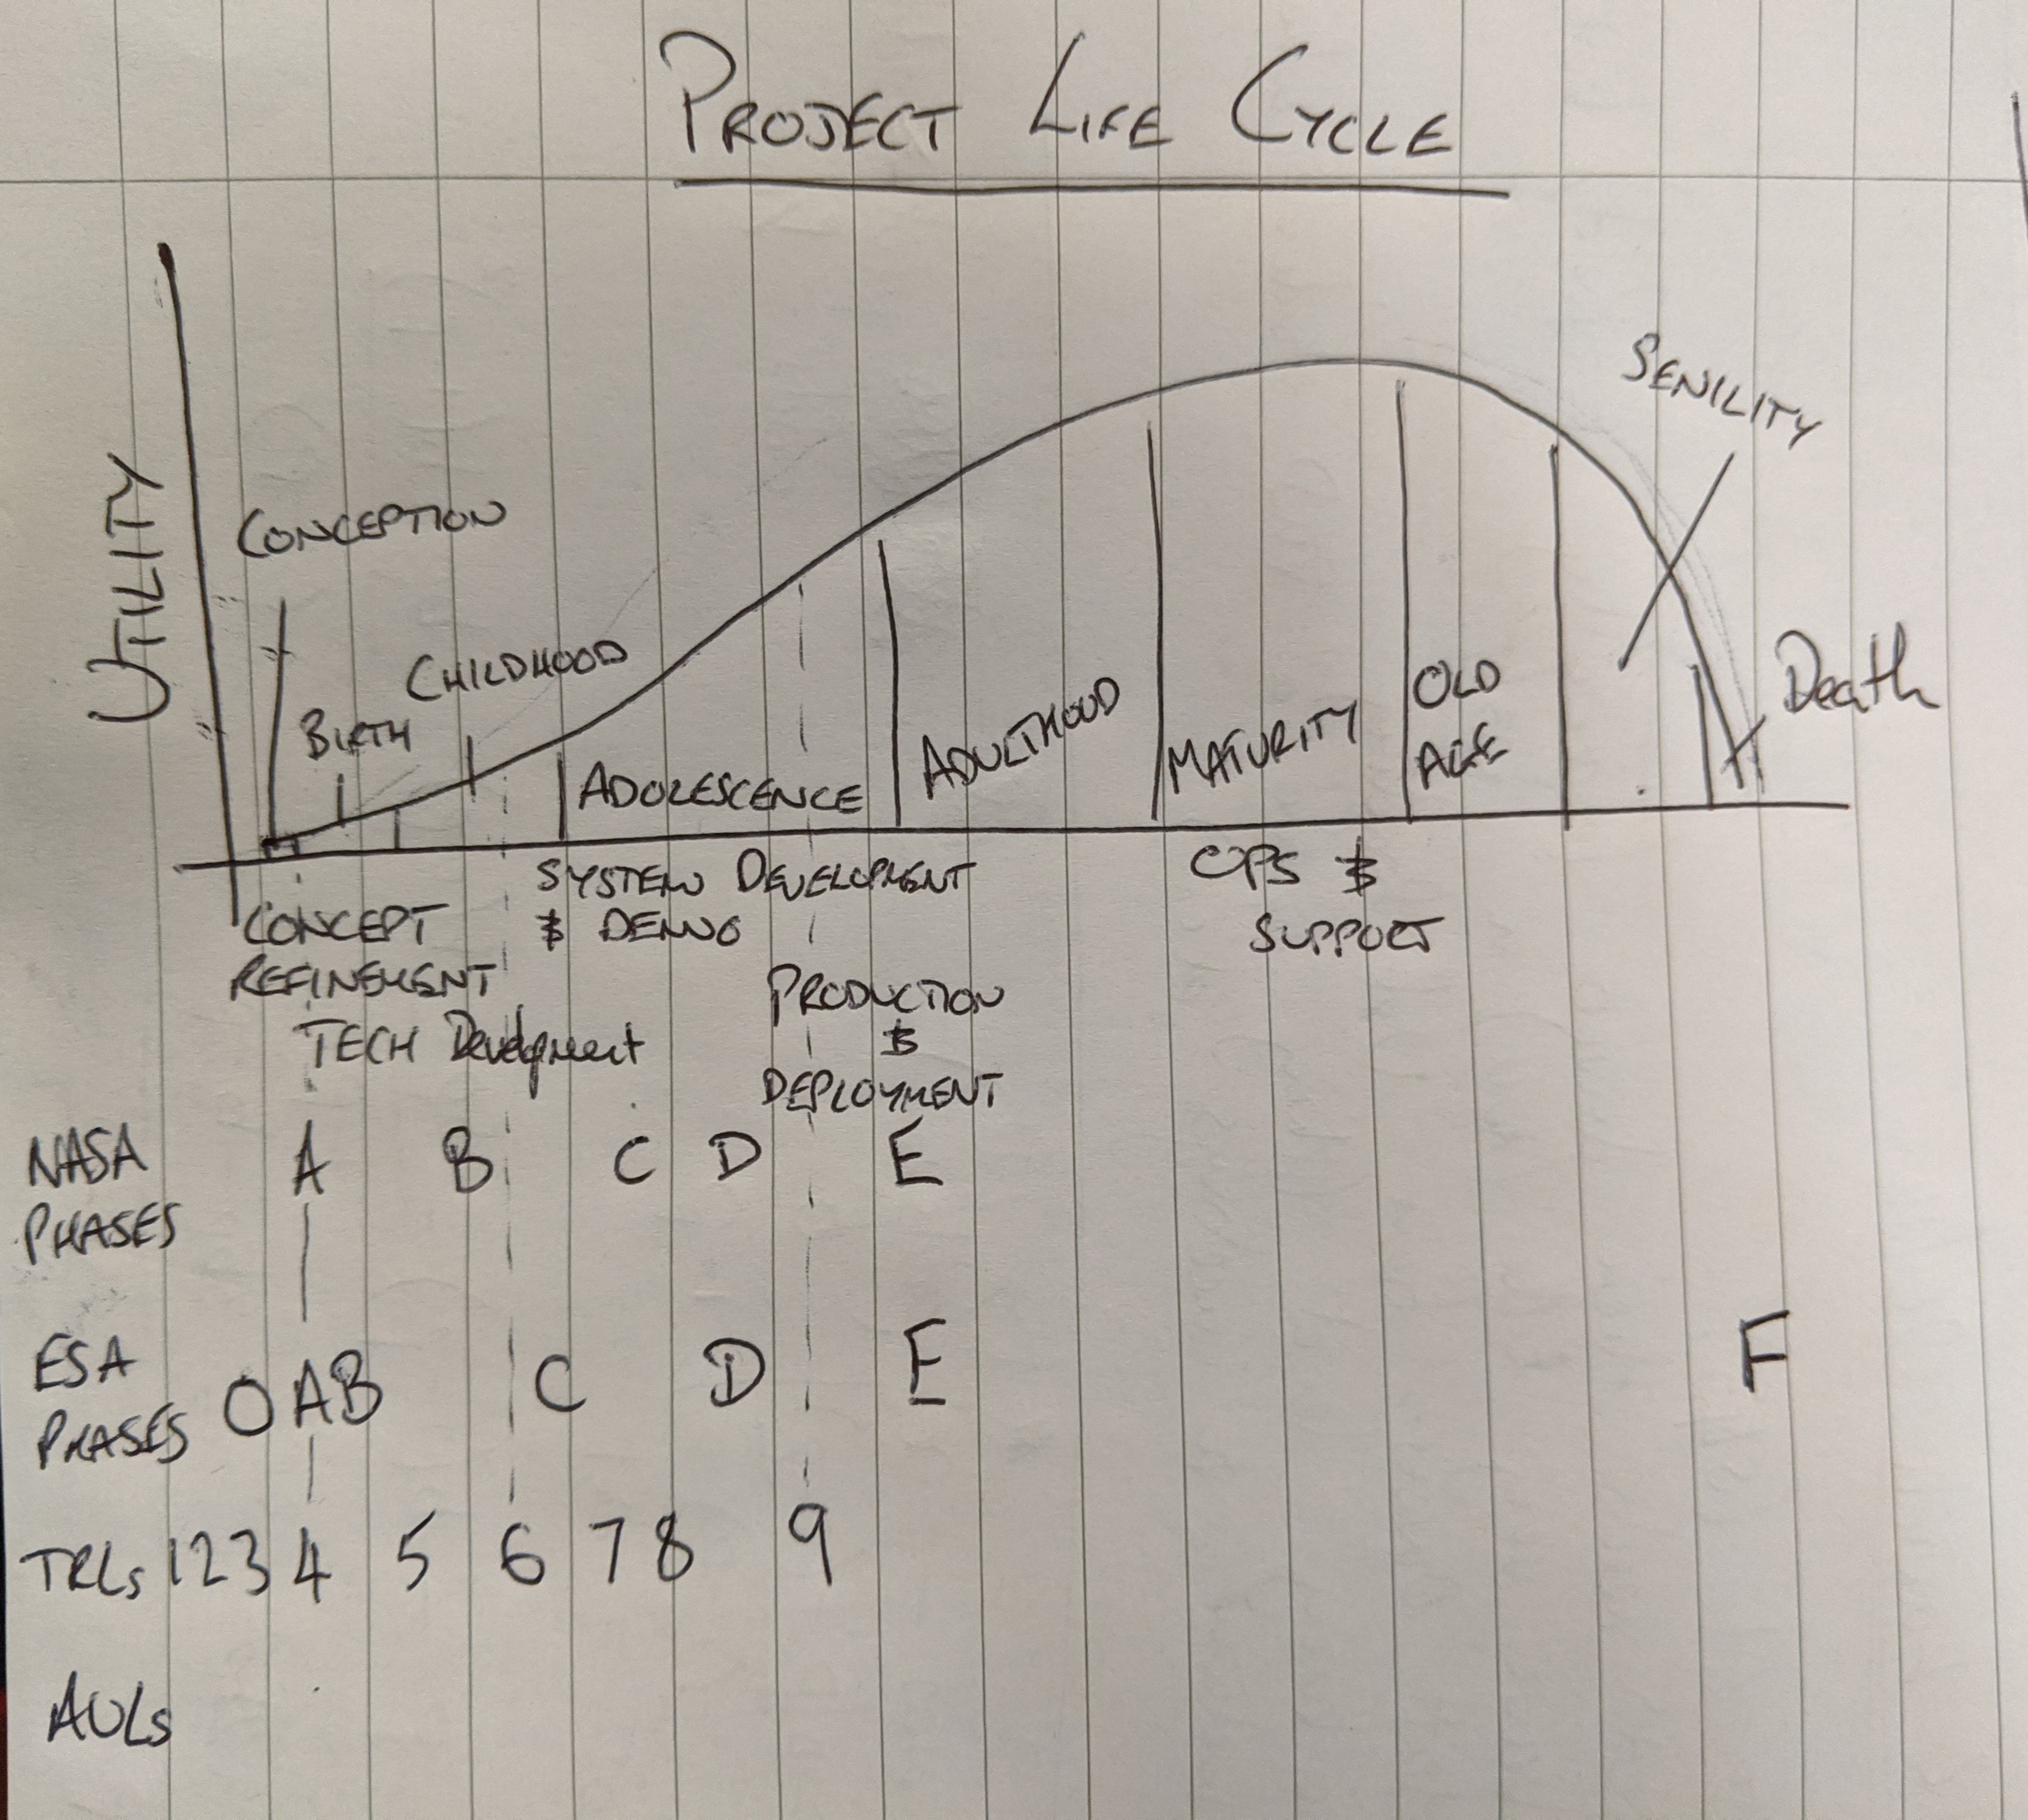
\includegraphics[scale=0.1]{whaleChart_hand.jpg}
    \caption{Hand drawn whale chart}
    \label{fig:whaleChart}
\end{figure}


\annote[Jeff]{The final operational version of the technology is thoroughly demonstrated through normal operations, with only minor problems needing to be fixed.}{Where does space flight fit into the AUL framework?  My reading of the above milestones seems like it would be lower than 9.  For instance, "sustained and repeated use" implies to me that this is after cal/val.} Any further improvements to the technology at this point, whether planned or not, will be treated as a TRL or AUL 1.

\subsection{at least one software project}
\subsubsection{sami2py and growin}
The sami2py software package \cite{sami2py}
\begin{figure}[h!t]
    \centering
    \includegraphics[width=0.9\textwidth]{sami2py_diagram.png}
    \caption{Block diagram of the sami2py ecosystem}
    \label{fig:whaleChart}
\end{figure}

\subsection{A flight software project}

\subsection{Maybe an example of how a funding program can use the AULs? }

\subsection{Edge cases?}
\annote[Jeff]{An area for the cases that fit in between TRL / AUL levels.}{Part of this is just me wondering where these would fit in.  Some of these are based on anecdotal stories of past missions.}  Possibilities:
\begin{itemize}
    \item A mission that has launched but is still under ``commissioning''
    \annote[Alexa]{For the application of successfully launched and operating in space, the mission is at an AUL 9. However, for the application of providing science quality data, the mission may only be at an AUL of 6 as the instrumentation is currently being validated in the real world environment.}{I think this would be right but not sure. }
    \item A mission that has one orbit of successful data, followed by fault through an unrelated subsystem (say, telemetry)
    \annote[Alexa]{For the application of delivering the satellite to the proper orbit the mission is at an AUL 9. However, for providing science data perhaps it is only at a TRL 8 in that validation was completed but sustained use is not achieved. }
    \item A mission with sporadic data due to tumbling spacecraft
    \annote[Alexa]{Like the previous two I think it reaches something in phase III, but perhaps it needs a new "branch" with new requirements. Perhaps the data is still usable in some format and new requirements are needed to fully state what the data quality that can be achieved is.  }
\end{itemize}

\section{Conclusions}

\annote[Alexa]{We need to also address/include what issues there are with the AULs that perhaps the TRLs or other frameworks address. }


\begin{acknowledgements}
      Part of this work was completely volunteer time by the co-authors. Other parts of this work were supported by...
\end{acknowledgements}

%%    This version assumes use of bibtex with the swsc.bib file being present
%%    If your bib file has a different name you need to change the following line

\bibliography{swsc}
   
\end{linenumbers}

\end{document}

